\documentclass[12pt, letterpaper]{article}
\usepackage[utf8]{inputenc}
\usepackage[margin=1in]{geometry}
\usepackage{booktabs}
\usepackage{tabu}
\usepackage[labelfont=bf, skip=5pt, font=small]{caption}
\usepackage{subcaption}
\usepackage{graphicx}
\usepackage{fancyhdr}
\usepackage{float}
% \usepackage[style=ieee, articletitle=true]{biblatex}
% \addbibresource{references.bib}



\setlength{\parskip}{1em}
\setlength{\parindent}{0em}


\begin{document}
\begin{center}
    \huge{Introduction to KUKA LBR iiwa Robotic Manipulators} \\[10pt]
    \large{Zachary Morin-Barich}
\end{center}









\section{Introduction}

This is a manual intended to bring the user up to date on the use of the KUKA LBR iiwa Robotic Manipulator. This document outlines the key steps in order to begin the project from scratch. First, a brief history of the project will be given, which will outline the steps that were taken to reach the present state of the project. The hardware set-up will then be discussed, which covers various topics such as safety procedures when working with the robots and the SmartPAD. The software set-up will also be discussed, which includes topics such as Workbench and ROS installations, Safety and IP configurations and programs. Lastly, the use of ROS and its applications will be discussed, as well as ROS basics, coding in ROS, sending commands and simulation.





\section{History}










\section{Hardware Set-Up}
\subsection{Safety}
It is imperative that a standard of safety is maintained when working with and around the robotic manipulators. Lack of such safety can result in injury and serious bodily harm. There are several safety factors which must be noted, such as:

\begin{itemize}
    \item All personnel must remain outside of the workspace of the robots;
    \item There are orange indicator lamps which indicate the cabinet health (not currently in use);
    \item There are 3 emergency stops;
    \begin{itemize}
        \item There is an e-stop on each SmartPAD;
        \item There is a desk-mounted e-stop which takes 1-2 seconds to halt motion;
    \end{itemize}
    \item There is an enabling switch which is required to be turned on or pressed in order to commence operation of the robot (not currently in use).
\end{itemize} 

\begin{figure}[!h]
    \centering
    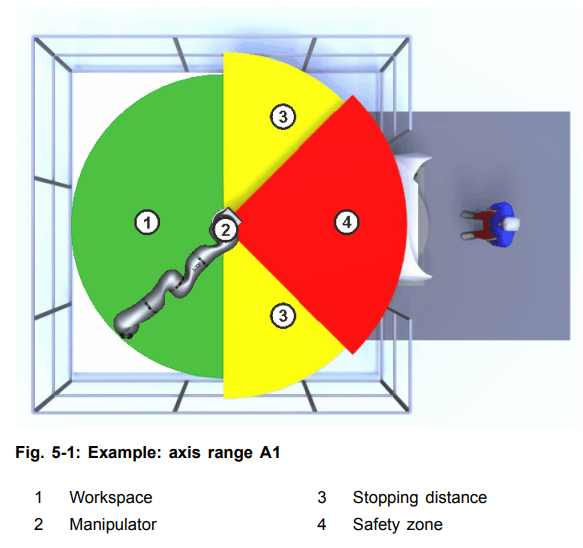
\includegraphics{Images/KUKAWorkspace.png}
    \caption{Example of robot's workspace \cite{}}
    \label{fig:robot-workspace}
\end{figure}

\textbf{Using the e-stop:}
\begin{itemize}
    \item Depressing the red e-stop button (either desk-mounted or on SmartPAD), twist clockwise to resume.
\end{itemize}
     
\textbf{X11 Port}
\begin{itemize}
    \item Port which connects the cabinets to the desk-mounted e-stop. 
    \item Purchased a Male DB50 Solderless Connector to complete safety circuit, as shown in Figure \ref{fig:safety-circuit-wiring}.
    \item This wiring was done in reference to the safety circuit provided by a KUKA representative, as shown in Figure \ref{fig:kuka-physical-circuit}.
\end{itemize}

\begin{figure}
    \centering
    \begin{subfigure}[b]{0.32\textwidth}
        \centering
        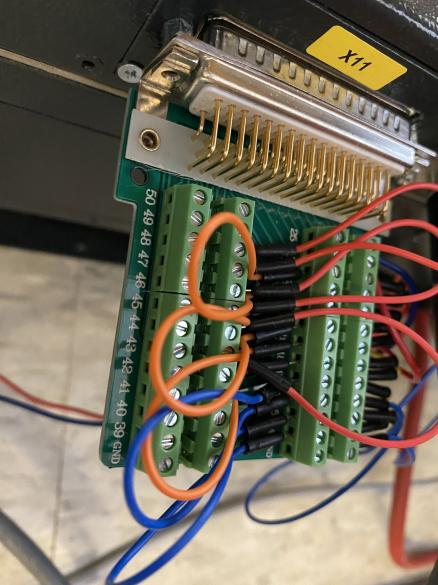
\includegraphics[width=\textwidth]{Images/IMG_1578.jpg}
        \caption{Left Side}
        \label{fig:safcl}
    \end{subfigure}
    \hfill
    \begin{subfigure}[b]{0.32\textwidth}
        \centering
        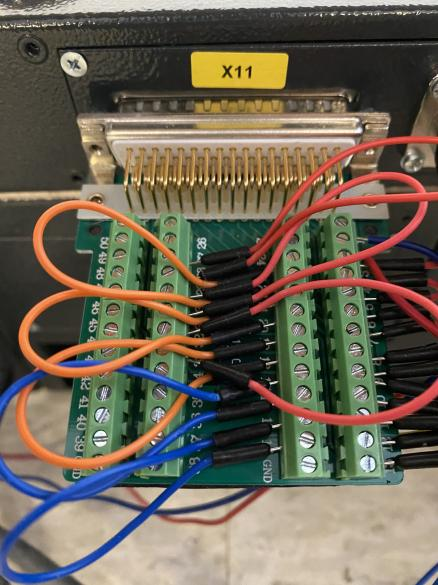
\includegraphics[width=\textwidth]{Images/IMG_1577.jpg}
        \caption{Top}
        \label{fig:safcc}
    \end{subfigure}
    \hfill
    \begin{subfigure}[b]{0.32\textwidth}
        \centering
        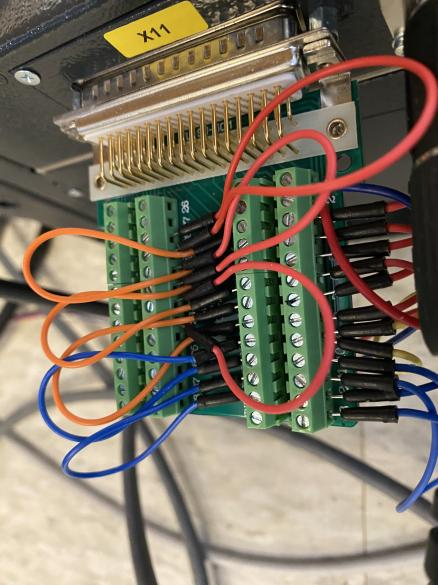
\includegraphics[width=\textwidth]{Images/IMG_1574.jpg}
        \caption{Right Side}
        \label{fig:safcr}
    \end{subfigure}
    \caption{Views of the Safety Circuit Wiring}
    \label{fig:safety-circuit-wiring}
\end{figure}

\begin{figure}[H]
    \centering
    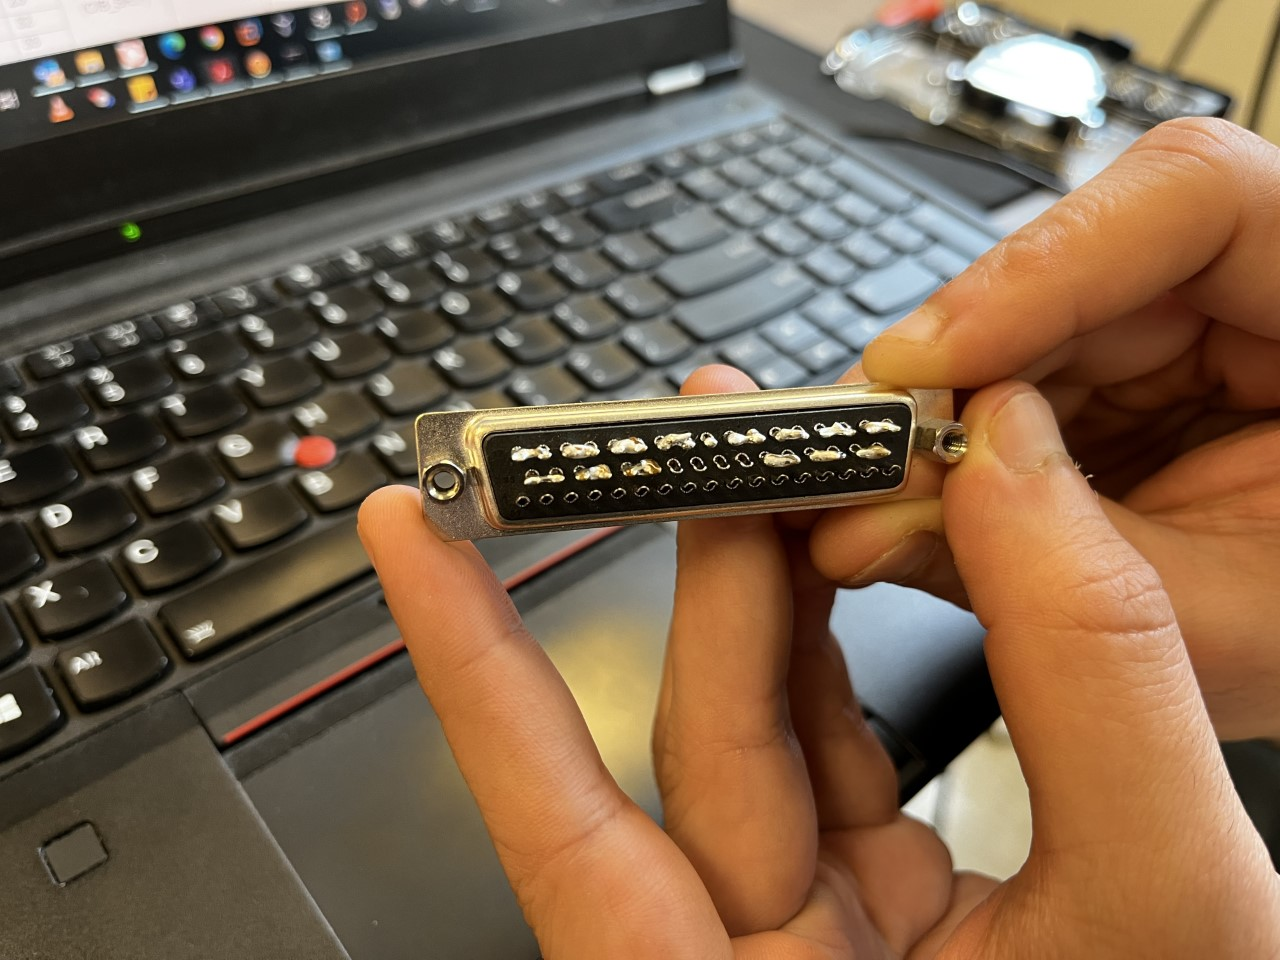
\includegraphics[width=\textwidth]{Images/Physical Circuit.jpg}
    \caption{Safety Circuit Wiring by KUKA Representative}
    \label{fig:kuka-physical-circuit}
\end{figure}




\subsection{SmartPAD}

\subsubsection{Jogging (Joint and Task Space)}


\textbf{Jogging in Joint Space} 

Move arm through changing individual joint angles. (Buttons found in Figure \ref{fig:SmartPADJoggingButtons})

\begin{itemize}
    \item Turn Mode Selector Switch
    \item Select T1 (Test mode 1, Reduced velocity)
    \item Return Mode Selector Switch to default position
    \item Depress Enabling Switch (1st indent to enable, 2nd indent will stop robot)
    \item While holding Enabling Switch, press Jog Keys for respective joints.
\end{itemize}

\textbf{Jogging in Task Space} 

Move arm through changing end effector positions. (Buttons found in Figure \ref{fig:SmartPADJoggingButtons})


\begin{itemize}
    \item Turn Mode Selector Switch
    \item Select T1 (Test mode 1, Reduced velocity)
    \item Return Mode Selector Switch to default position
    \item Depress Enabling Switch (1st indent to enable, 2nd indent will stop robot)
    \item While holding Enabling Switch, press Jog Keys for desired motion.
        \begin{itemize}
            \item X, Y, Z = Linear Motion along respective axis.
        \end{itemize}
        \begin{itemize}
            \item A, B, C = Rotational Motion along Z, Y, X axis, respectively.
        \end{itemize}
        \begin{itemize}
            \item R = null space of robot (end effector does not move) using elbow
        \end{itemize}
    \item Beware of positions that will result in singularities when working in Task Space. When a singularity is reached, no motion can occur in that direction. 
\end{itemize}

Additional information about moving the robots can be found in Figure \ref{fig:KUKAJointAngleDepiction}.


\begin{figure}[h!]
    \centering
    \begin{subfigure}[b]{0.32\textwidth}
        \centering
        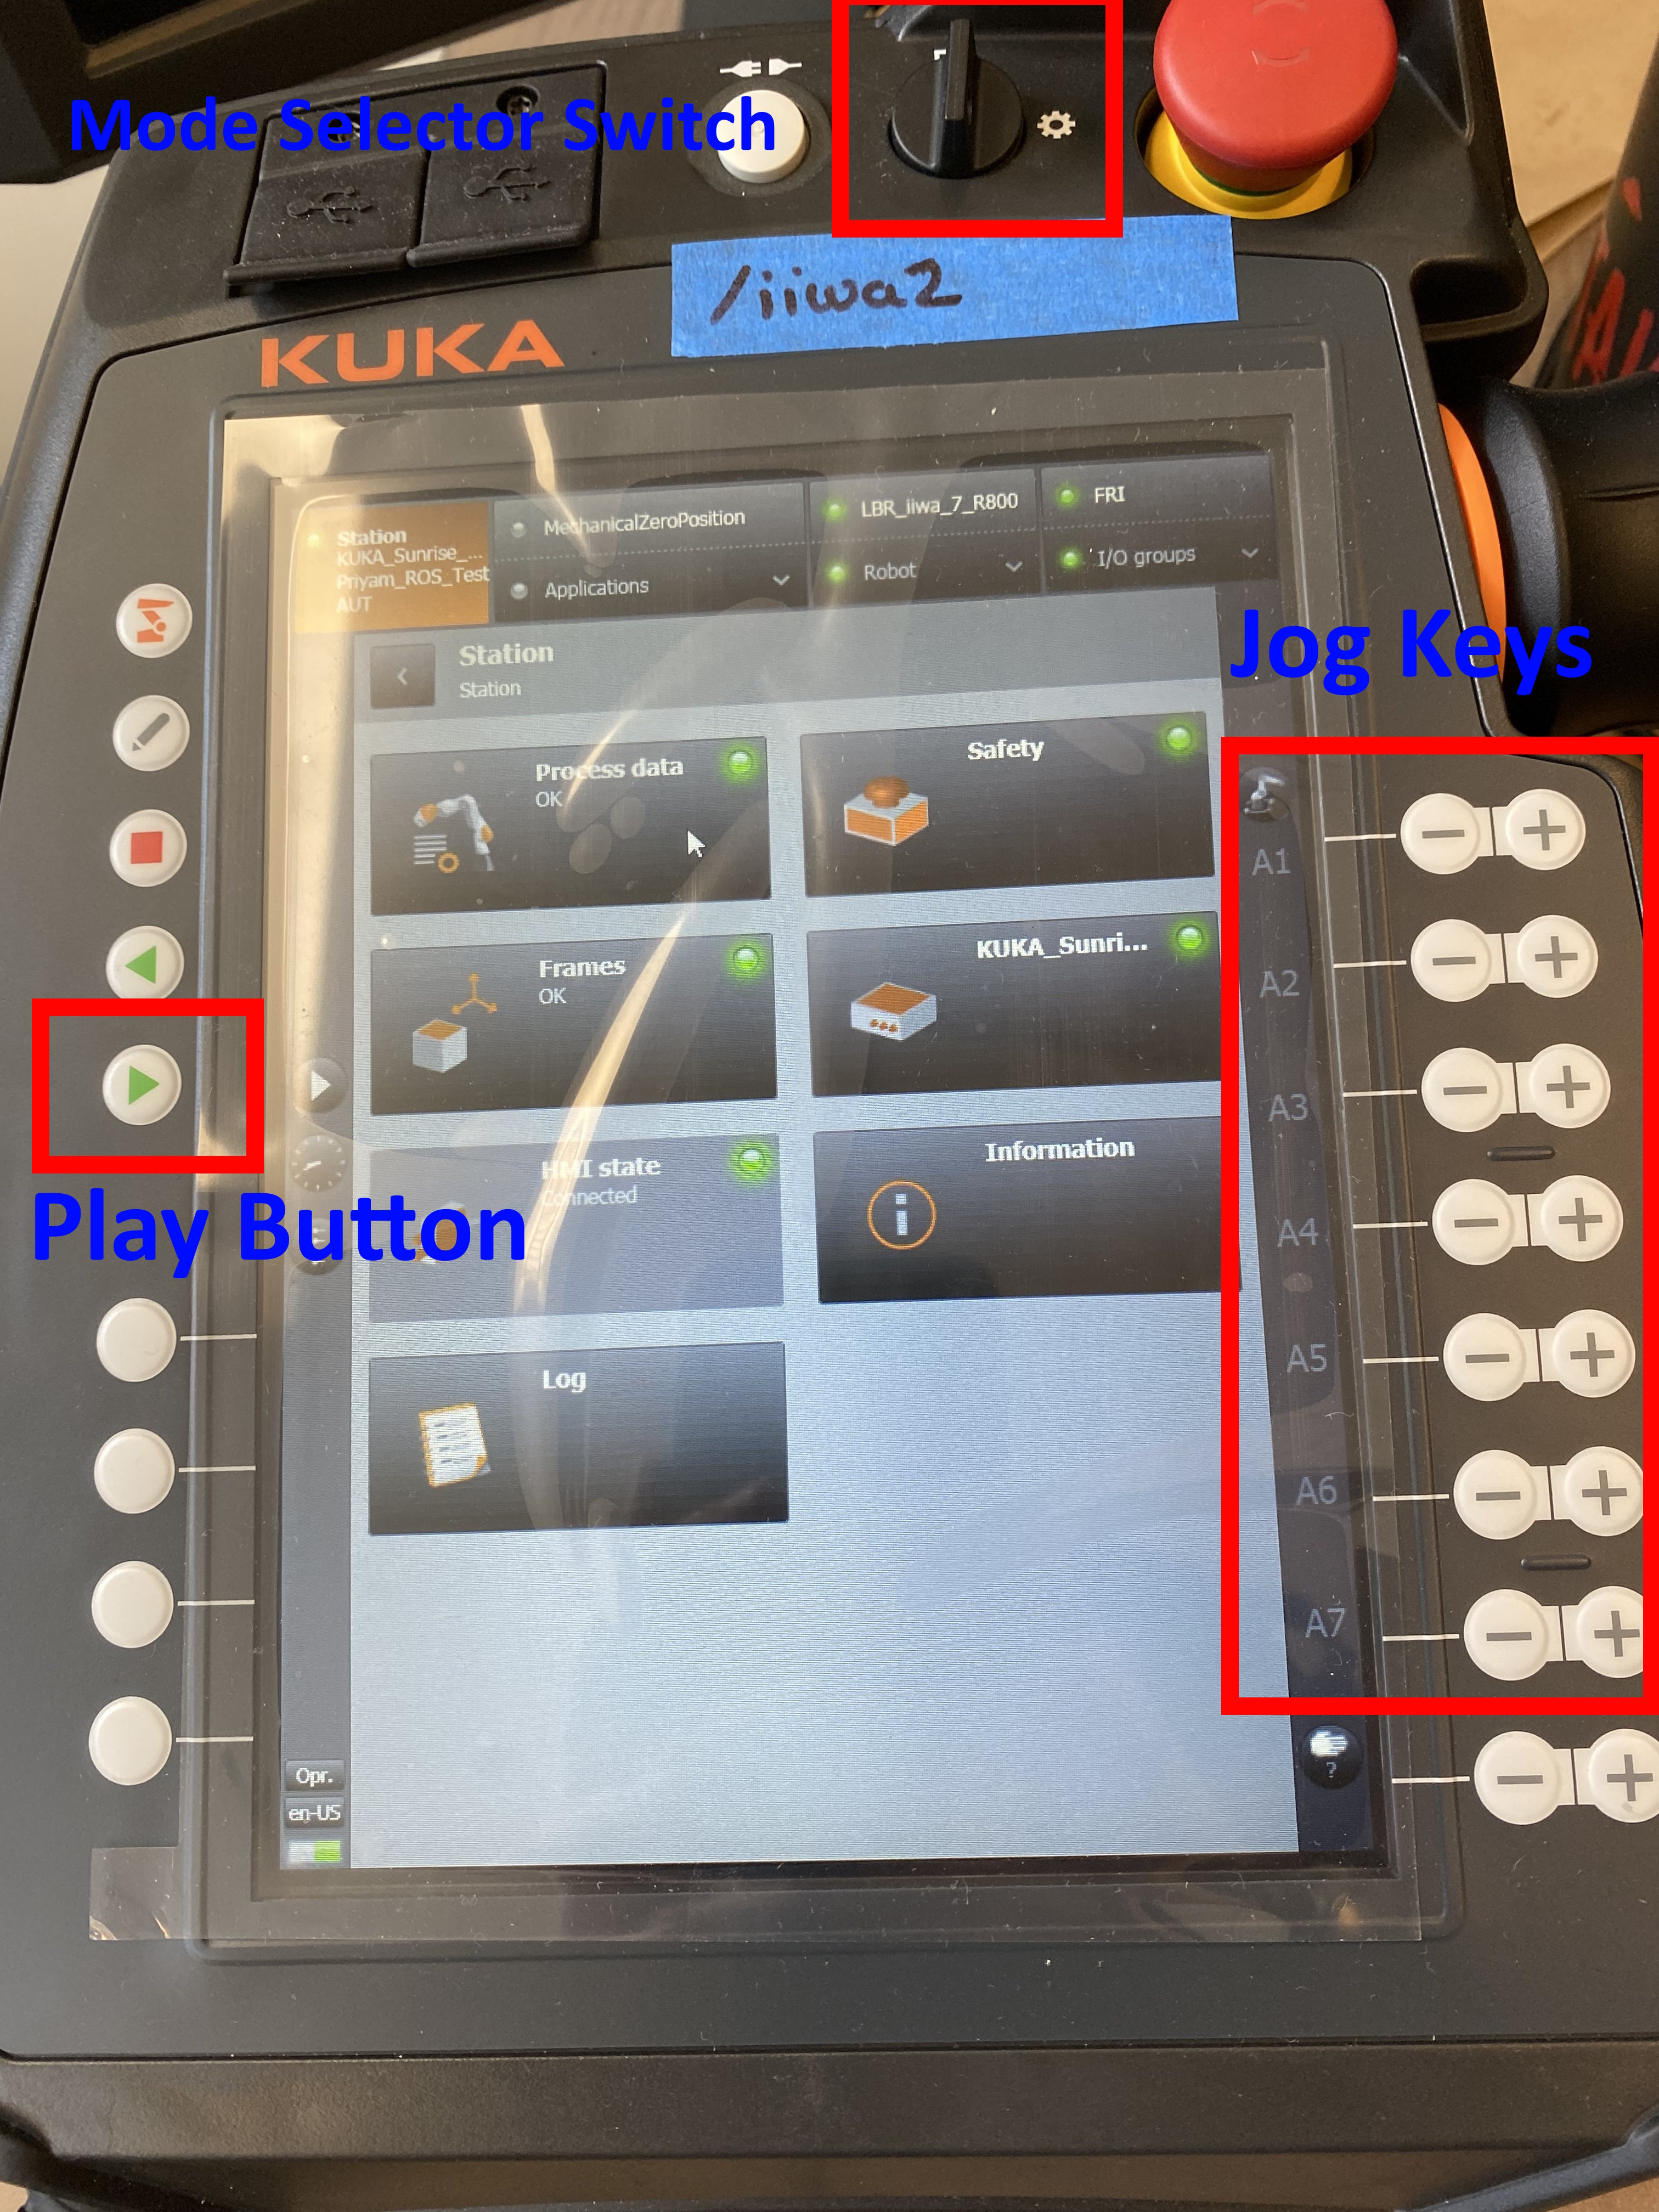
\includegraphics[width=\textwidth]{Images/ImportantButtonsFront.jpg}
        \caption{}
        \label{fig:buttonsfront}
    \end{subfigure}
    \hfill
    \begin{subfigure}[b]{0.32\textwidth}
        \centering
        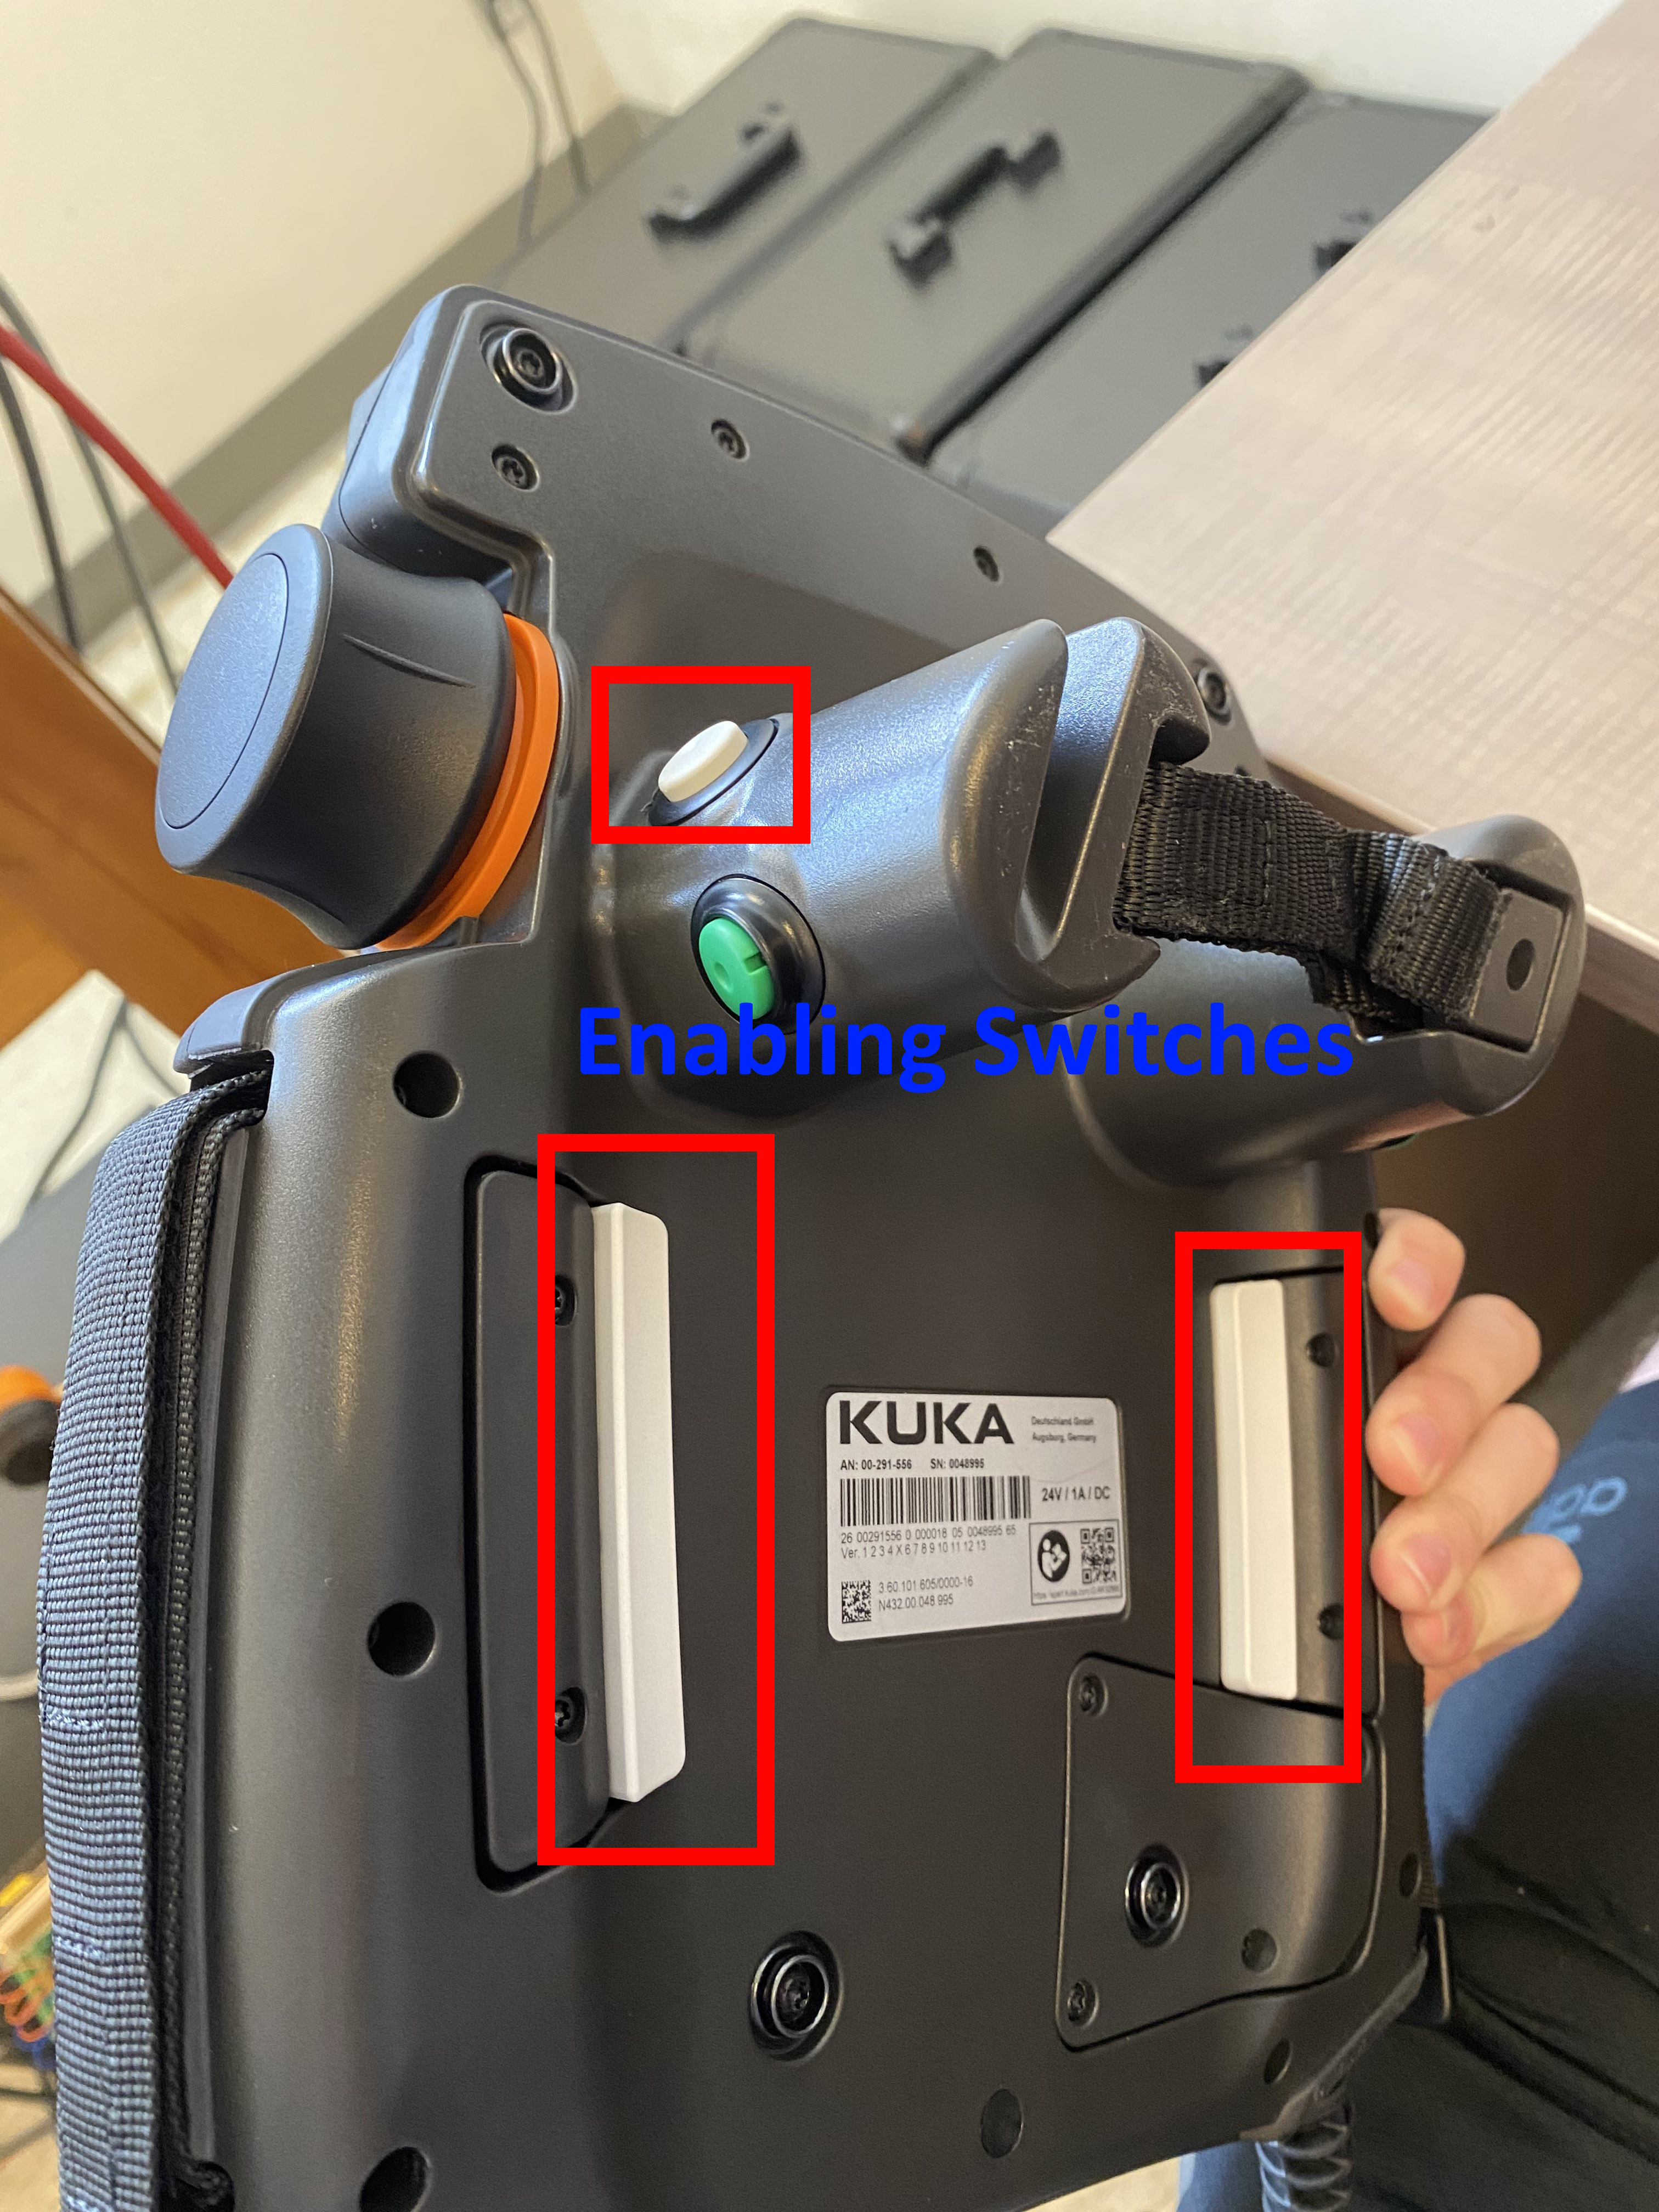
\includegraphics[width=\textwidth]{Images/ImportantButtonsBack.jpg}
        \caption{}
        \label{fig:buttonsback}
    \end{subfigure}
    \hfill
    \begin{subfigure}[b]{0.32\textwidth}
        \centering
        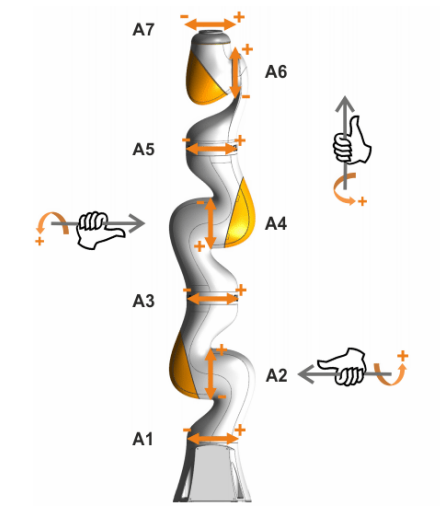
\includegraphics[width=\textwidth]{Images/KUKAJointAngles.png}
        \caption{}
        \label{fig:KUKAJointAngleDepiction}
    \end{subfigure}
    \caption{Important SmartPAD Information}
    \label{fig:SmartPADJoggingButtons}
\end{figure}




% singularities (task space), null space


\subsubsection{Applications}
\textbf{Viewing Applications}
\begin{itemize}
    \item Find the "Applications" tab in the Navigation bar (See Figure \ref{fig:SmartPAD-NavnApp})
    \item Press on the tab. All applications will be displayed on the screen, as shown in Figure \ref{fig:SmartPADApplications1} and \ref{fig:SmartPADApplications2}.
\end{itemize}


\begin{figure}[h!]
    \centering
    \begin{subfigure}[b]{0.32\textwidth}
        \centering
        \includegraphics[width=\textwidth]{Images/SmartPADHomeScreen.jpg}
        \caption{}
        \label{fig:SmartPAD-NavnApp}
    \end{subfigure}
    \hfill
    \begin{subfigure}[b]{0.32\textwidth}
        \centering
        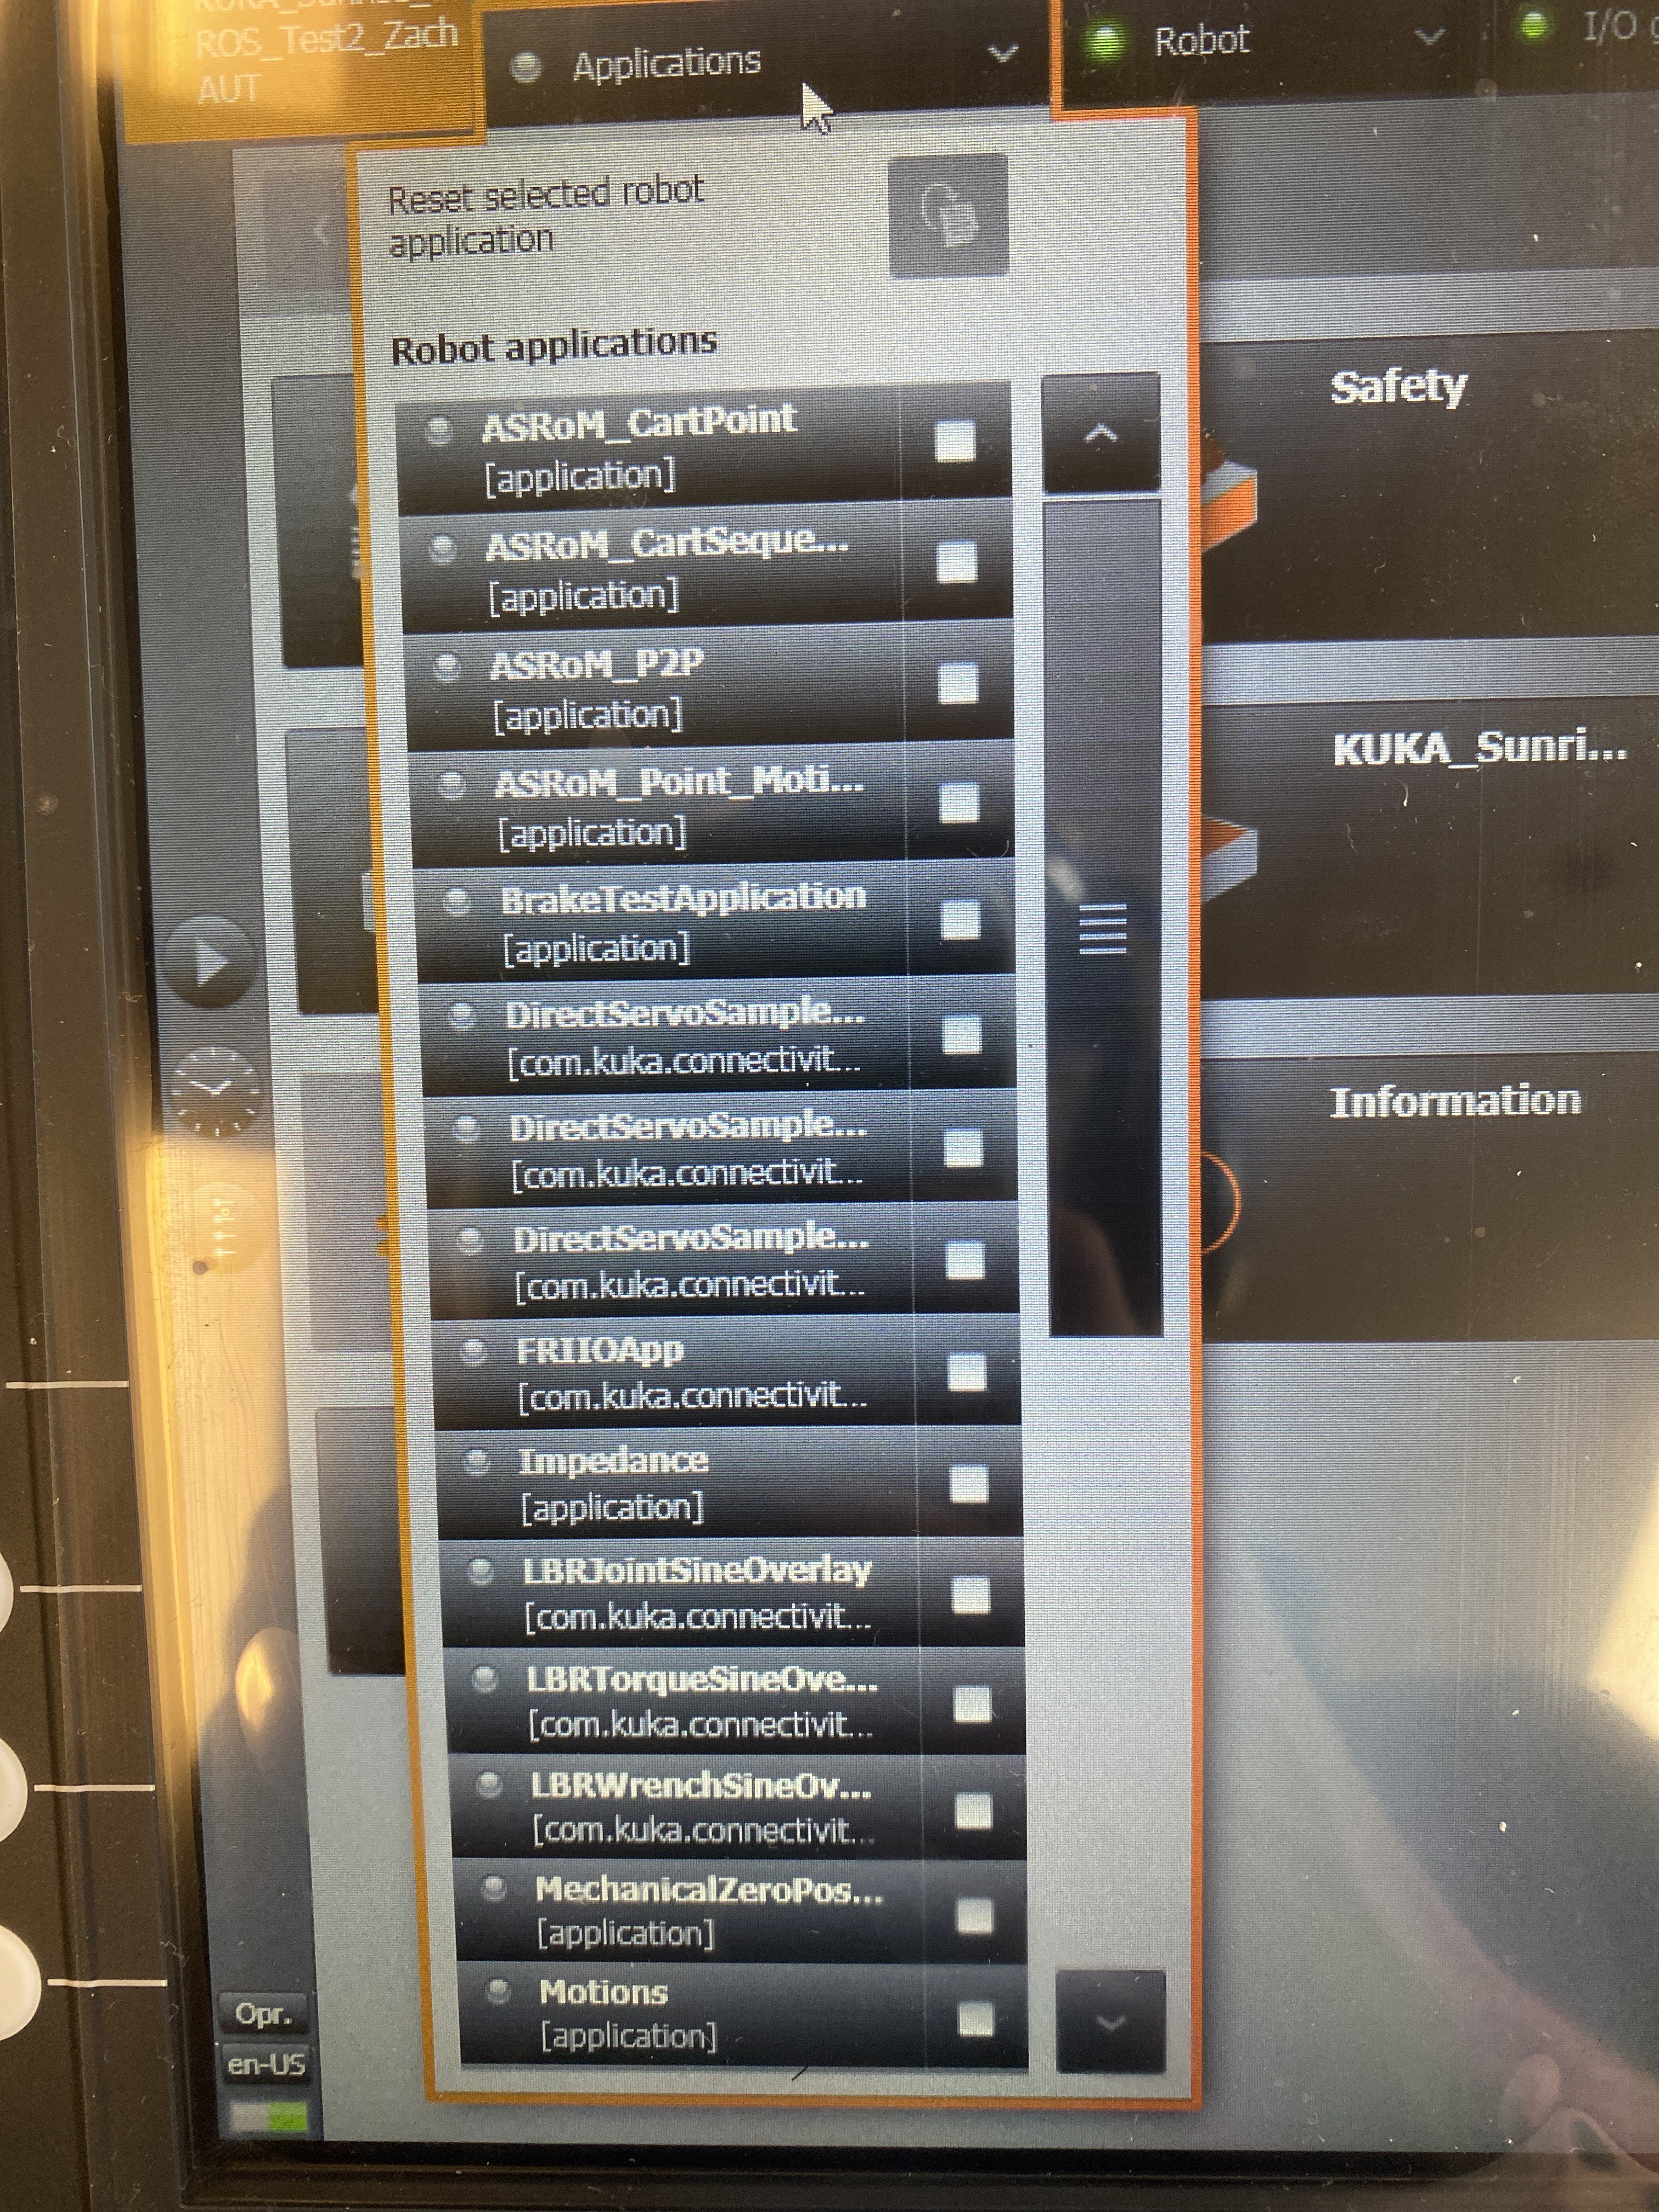
\includegraphics[width=\textwidth]{Images/SmartPAD Applications1.jpg}
        \caption{}
        \label{fig:SmartPADApplications1}
    \end{subfigure}
    \hfill
    \begin{subfigure}[b]{0.32\textwidth}
        \centering
        \includegraphics[width=\textwidth]{Images/SmartPAD Applications2.jpg}
        \caption{}
        \label{fig:SmartPADApplications2}
    \end{subfigure}
    \caption{Navigation Tab with Applications Tab and Available Applications on the SmartPAD}
    \label{fig:SmartPADPrograms}
\end{figure}


\textbf{Running Applications}

\begin{itemize}
    \item Press on the required application.
    \item Press down on one of the enabling switches.
    \item Press the green Play button.
    \item If in automatic mode, let go of the enabling switch. 
\end{itemize}


\subsubsection{Reading Sensors}

\textbf{Reading torque, axis and Cartesian positions}

\begin{itemize}
    \item From the home-screen, press on the tab which indicates the name of the robot.
    \item Data can be read from 3 separate programs (Seen in Figure \ref{fig:SensorReading})
\end{itemize}


\begin{figure}[H]
    \centering
    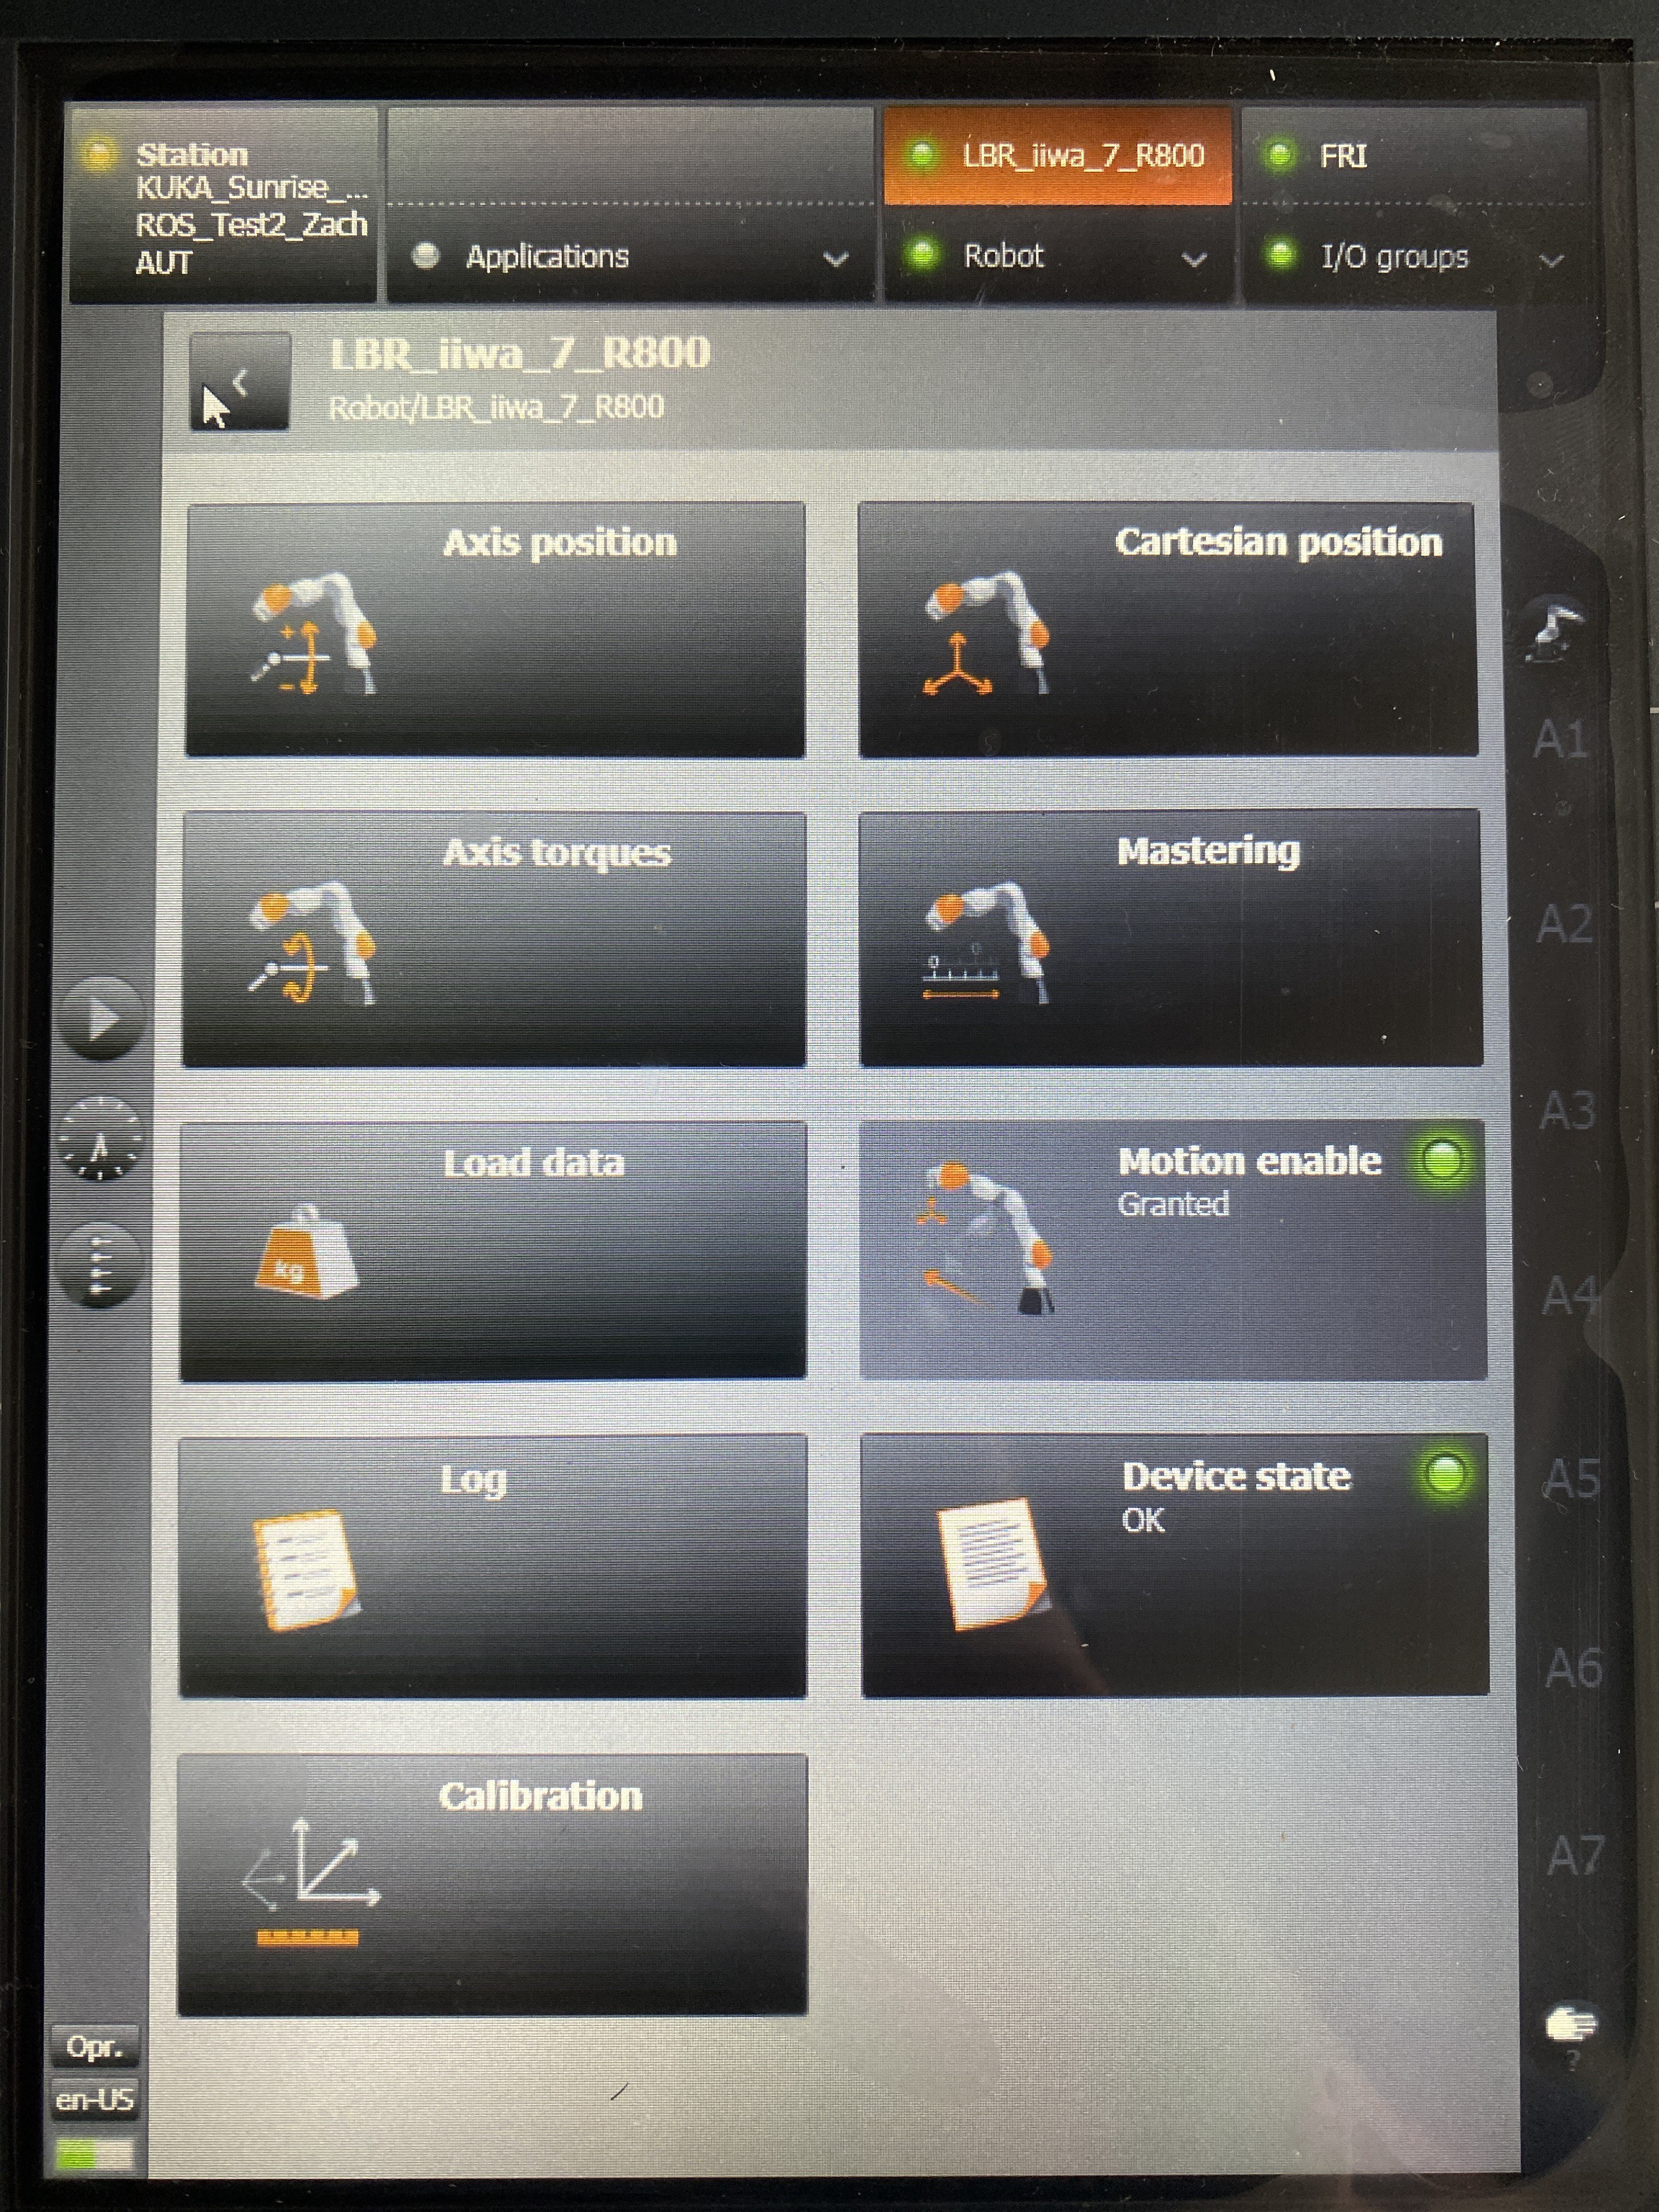
\includegraphics[scale=0.08]{Images/SmartPAD Readings.jpg}
    \caption{Programs which allow the user to read the data from the robot.}
    \label{fig:SensorReading}
\end{figure}






\section{Software Set-Up}
\subsection{KUKA Sunrise Workbench}
\subsubsection{Installation}
% Simple install? Files found in USB I think? If not, on PC. Unsure, cannot elaborate. Also unsure of setting up packages. 
\subsubsection{Connect To Robot}
\begin{itemize}
    \item Connect PC to the cabinet with ethernet cable through the X66 port, located above the power switch.
    \item In order to communicate, both PC and cabinet must be on the same subnets. 
\end{itemize}
\subsubsection{Station Setup}
% Under ROSJavaLib
\begin{itemize}
    \item Click on "StationSetup.cat".
    \item 3 options; Software, Configuration, Installation
    \item Software permits choice of pre-made software installed onto cabinet
    \item Configuration is where the IP addresses can be changed, as well as the Subnet masks. Verify documentation before changing values.
    \item Lastly, installation tab allows to install the desired station configuration.
\end{itemize}
\subsubsection{Deploying A Program}
\begin{itemize}
    \item Press on the "Synchronize project" button in Workbench under the "ROSJavaLib" folder. 
    \item Will prompt to execute synchronization. Can load to controller or load from controller. 
    \item In order to function properly, IP addresses must be configured proplerly. 
\end{itemize}
\subsubsection{Safety Configuration}
% Under ROSJavaLib
\begin{itemize}
    \item Also in the "ROSJavaLib" folder.
    \item Allows for the configuration of various safety parameters for the robots.
\end{itemize}









\subsection{ROS}
\subsubsection{Installation}

\subsubsection{MoveIt}

\subsubsection{Connecting ROS Machine to Cabinet}

%IPs n naming 









\section{ROS Application}
\subsection{ROS Nodes}

\subsection{ROSSmartServo}

\subsection{ROS Message Classes}

\subsection{Coding the Commands}

\subsection{Joint Position Commands}

\subsection{Sending A Command}

\subsection{Gazebo}

\subsection{URDF}








\end{document}